\documentclass[spanish, 12pt]{exam}

%These tell TeX which packages to use.
\usepackage{array,epsfig}
\usepackage{amsmath}
\usepackage{amsfonts}
\usepackage{amssymb}
\usepackage{amsxtra}
\usepackage{amsthm}
\usepackage{mathrsfs}
\usepackage{color}
\usepackage{multicol}
\usepackage{verbatim}

\usepackage[utf8]{inputenc}
\usepackage[spanish]{babel}
\usepackage{eurosym}

\usepackage{graphicx}
\graphicspath{{../img/}}

\printanswers
\nopointsinmargin
\pointformat{}

%Pagination stuff.
%\setlength{\topmargin}{-.3 in}
%\setlength{\oddsidemargin}{0in}
%\setlength{\evensidemargin}{0in}
%\setlength{\textheight}{9.in}
%\setlength{\textwidth}{6.5in}
%\pagestyle{empty}

\renewcommand{\solutiontitle}{\noindent\textbf{Sol:}\enspace}

\newcommand{\class}{4º Académicas}
\newcommand{\examdate}{\today}
\newcommand{\examnum}{Ecuaciones y sistemas}
\newcommand{\tipo}{A}


\newcommand{\timelimit}{50 minutos}



\pagestyle{head}
\firstpageheader{
\includegraphics[width=0.2\columnwidth]{header_left}}{\textbf{Departamento de Matemáticas\linebreak \class}\linebreak \examnum}{
\includegraphics[width=0.1\columnwidth]{header_right}}
\runningheader{\class}{\examnum}{Página \thepage\ of \numpages}
\runningheadrule

\begin{document}

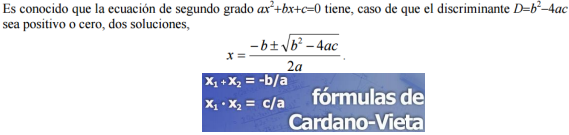
\includegraphics[width=0.9\columnwidth]{ec2grado}

\begin{questions}


\question Dadas las siguientes ecuaciones se pide:
\begin{itemize}
\item Resolverlas mediante la fórmula general de la ecuación de segundo grado
\item Comprobar las soluciones obtenidas
\item Factorizar el polinomio del primer miembro de cada ecuación
\item Comprobar las relaciones de Cardano-Vieta
\end{itemize}

\begin{multicols}{3}
\begin{parts}
\part[] $x^2-4x+3=0$ 

\begin{solution} \end{solution}

\part[] $x^2-5x+6=0$ 
\begin{solution} \end{solution}

\part[] $x^2+2x+5=0$ 
\begin{solution} \end{solution}

\part[] $2x^2-5x+2=0$ 
\begin{solution} \end{solution}

\part[] $6x^2-13x+6=0$ 
\begin{solution} \end{solution}

\part[] $x^2-4x+3=0$ 
\begin{solution} \end{solution}


\end{parts}
\end{multicols}

\question Escribir \emph{una} ecuación de 2º grado que tenga por soluciones.
\begin{multicols}{3}
\begin{parts}
\part[] $x_1=4 $, $x_2=-6$ 
\begin{solution} $x^2+2x-24=0$ \end{solution}

\part[] $x_1=-3 $, $x_2=-5$ 
\begin{solution} $x^2+8x+15=0$ \end{solution}

\part[] $x_1=2 $, $x_2=-7$ 
\begin{solution} $x^2+5x-14=0$ \end{solution}

\part[] $x_1=-2/7 $, $x_2=7$ 
\begin{solution} $7x^2-47x-14=0$ \end{solution}

\part[] $x_1=-16 $, $x_2=9$ 
\begin{solution} $x^2+7x-144=0$ \end{solution}

\part[] $x_1=-4 $, $x_2=-1/8$ 
\begin{solution} $8x^2+33x+4=0$ \end{solution}

\part[] $x_1=2 $, $x_2=-2$ 
\begin{solution} $x^2-4=0$ \end{solution}

\part[] $x_1=\sqrt{2} $, $x_2=-\sqrt{2}$ 
\begin{solution} $x^2-2=0$ \end{solution}

\part[] $x_1=2/5 $, $x_2=2/5$ 
\begin{solution} $25x^2-20x+4=0$ \end{solution}

\part[] $x_1=2+\sqrt{3} $, $x_2=2-\sqrt{3}$ 
\begin{solution} $x^2-4x+1=0$ \end{solution}

\end{parts}
\end{multicols}

\question ¿Para qué valores de \emph{a} la ecuación $x^2-6x+3+a=0$ tiene solución única? 
%\begin{multicols}{3}
\begin{solution} $a=-6 $\end{solution}
%\end{multicols}

\question Resolver las siguientes ecuaciones de \textbf{2º grado incompletas}:
\begin{multicols}{4}
\begin{parts}
\part[] $x^2-5x=0$  
\begin{solution} $x_1=0$, $x_2=5$ 
\end{solution}

\part[] $2x^2-6x=0$  
\begin{solution} $x_1=0$, $x_2=3$ 
\end{solution}

\part[] $2x^2-18=0$  
\begin{solution} $x_1=3$, $x_2=-3$ 
\end{solution}

\part[] $5x^2+x=0$  
\begin{solution} $x_1=0$, $x_2=-1/5$ 
\end{solution}

\part[] $x^2=x$  
\begin{solution} $x_1=0$, $x_2=2$ 
\end{solution}



\part[] $x^2+x=0$  
\begin{solution} $x_1=0$, $x_2=-1$ 
\end{solution}

\part[] $4x^2-1=0$  
\begin{solution} $x_1=1/2$, $x_2=-1/2$ 
\end{solution}

\part[] $-x^2+12x=0$  
\begin{solution} $x_1=0$, $x_2=12$ 
\end{solution}

\part[] $x^2-10x=0$  
\begin{solution} $x_1=0$, $x_2=10$ 
\end{solution}

\part[] $9x^2-4=0$  
\begin{solution} $x_1=2/3$, $x_2=-2/3$ 
\end{solution}

\end{parts}
\end{multicols}


\question Resolver las siguientes ecuaciones de \textbf{2º grado completas}:
\begin{multicols}{3}
\begin{parts}
\part[] $x^2-2x-8=0$  
\begin{solution} $x_1=4$, $x_2=-2$ 
\end{solution}

\part[] $2x^2-\sqrt{2} x-2=0$  
\begin{solution} $x_1=\sqrt{2}$, $x_2=-\sqrt{2}/2$ 
\end{solution}

\part[] $x^2+x+1=0$  
\begin{solution} $x_1=$, $x_2=$ 
\end{solution}

\part[] $x^2+x+1=0$  
\begin{solution} $x_1=$, $x_2=$ 
\end{solution}

\part[] $x^2+x+1=0$  
\begin{solution} $x_1=$, $x_2=$ 
\end{solution}

\part[] $x^2+x+1=0$  
\begin{solution} $x_1=$, $x_2=$ 
\end{solution}

\part[] $x^2+x+1=0$  
\begin{solution} $x_1=$, $x_2=$ 
\end{solution}

\part[] $x^2+x+1=0$  
\begin{solution} $x_1=$, $x_2=$ 
\end{solution}

\part[] $x^2+x+1=0$  
\begin{solution} $x_1=$, $x_2=$ 
\end{solution}

\part[] $x^2+x+1=0$  
\begin{solution} $x_1=$, $x_2=$ 
\end{solution}

\part[] $x^2+x+1=0$  
\begin{solution} $x_1=$, $x_2=$ 
\end{solution}

\part[] $x^2+x+1=0$  
\begin{solution} $x_1=$, $x_2=$ 
\end{solution}

\part[] $x^2+x+1=0$  
\begin{solution} $x_1=$, $x_2=$ 
\end{solution}

\part[] $x^2+x+1=0$  
\begin{solution} $x_1=$, $x_2=$ 
\end{solution}


\end{parts}
\end{multicols}

\begin{comment}
\question 
\begin{multicols}{3}
\begin{parts}
\part[]  
\begin{solution} \end{solution}

\end{parts}
\end{multicols}
\end{comment}

\end{questions}
\end{document}


